\documentclass[10pt]{article}
\usepackage[margin=2cm]{geometry}
\usepackage{amsmath,amssymb}
\usepackage{booktabs}
\usepackage{graphicx}
\usepackage{float}
\usepackage[font=small,labelfont=bf]{caption}
\usepackage[compact]{titlesec}
\usepackage{enumitem}
\usepackage{microtype}
\usepackage[hidelinks]{hyperref}
\setlist{itemsep=1pt,topsep=3pt}
\setlength{\parskip}{4pt}
\setlength{\parindent}{0pt}
\graphicspath{{figures/}}
\newcommand{\fig}[1]{Figure~\ref{#1}}
\newcommand{\tab}[1]{Table~\ref{#1}}

\begin{document}

\begin{center}
{\LARGE SuperMimic on Kangaroo, M2: the world model}\\[4pt]
Offline study of a learned dynamics model for PAL Kangaroo (7-DoF arms).
Branch \texttt{omm/supermimic} of pal\_mjlab, 23 October 2026.
\end{center}

\section*{Summary}

SuperMimic (arXiv 2610.28480) trains a motion-tracking policy by backpropagating through a learned
model of the robot's dynamics instead of through the simulator. Milestone M2 tested that model alone,
before any policy is trained on it. We fit the paper's world model, an MLP with three layers of 2048 units,
on 6.1M simulated Kangaroo transitions logged from our PPO baseline. Then we measured it on motion clips
it never saw during training.

\begin{itemize}
  \item \textbf{It predicts well up to the paper's horizon of 32 steps (0.64\,s).} Run open loop on
  recorded actions, the 14 tracked bodies are off by \textbf{0.86\,cm after 8 steps} and \textbf{3.8\,cm
  after 32 steps}. That is 4--6$\times$ below a baseline that predicts no motion. The imagined tracking
  return over 32 steps is within \textbf{1.1\%} of the real one. At 64 steps the error grows to 15\,cm,
  so 32 steps is about the useful limit.
  \item \textbf{Its gradients improve the real return.} A small change of the actions along the model's
  gradient raised the simulated return from \textbf{97--100\%} of the start states. Random changes of the
  same size did so from 44--47\%. Up to 16 steps the predicted gain matches the real one within 10\%. At
  32 steps the model is \textbf{optimistic}: it promises 1.3--1.6$\times$ the gain that is realized.
  \item \textbf{The paper's choices hold on Kangaroo.} Training on 8-step windows is essential: a model
  trained on single steps \emph{diverges} at 32 steps. Predicting state changes is $2\times$ better than
  predicting the next state. The full width of 2048 units is 15--20\% better than 1024. A policy the model
  never saw costs about 15\%.
  \item \textbf{The learned failure detector is the weak part.} It ranks failures with AUC 0.937, below
  our 0.95 gate. The simulator's own failure rule, applied to the model's predicted states, reaches 0.995.
\end{itemize}

\textbf{Recommendation for M3.} Use the main configuration (8-step training, $2048{\times}3$, delta
targets). In imagination, replace the learned failure head with a smooth version of the simulator's
failure rule. Log the imagined-vs-simulated return gap from the first iteration, because the model is
optimistic at 32 steps. Total GPU time for M2 was about 2.6\,h on the local RTX 5060 Ti.

\section{Why the world model is the main risk}

\textbf{The SuperMimic loop.} The paper repeats three steps (Alg.~A.1):
\begin{enumerate}
  \item \textbf{Collect} simulator transitions with the current policy plus Gaussian action noise
  $\mathcal N(0, 0.1^2)$, into a replay buffer.
  \item \textbf{Fit the world model} $f_\omega$ on short windows from the buffer (paper Eq.~1).
  \item \textbf{Train the policy} by imagining $H = 32$ steps with the model, from start states drawn
  from the buffer, and backpropagating the imagined return into the policy (paper Eq.~2). A critic
  $V$ estimates the return beyond the horizon (Eq.~3).
\end{enumerate}

\textbf{The imagined return.} With predicted states $\hat s$, reference goals $g$, rewards $r$ and a
survival weight $c$ that discounts states after a likely fall, the policy maximizes
\[
J(\theta) = \sum_{t=0}^{H-1} \gamma^t\, c_t\, r(\hat s_{t+1}, g_{t+1}) + \gamma^H c_H\, V(\hat s_H),
\qquad
\hat s_{t+1} = f_\omega\big(\hat s_t,\ \pi_\theta(o_t, g_t),\ \xi\big),
\qquad c_{t+1} = c_t\,(1 - \hat d_{t+1}),
\]
where $\xi$ is the episode's domain-randomization context (friction, calibration, centre of mass) and
$\hat d$ the predicted failure probability.

\textbf{Why this is the risk.} The gradient $\partial J/\partial\theta$ flows through every model step.
PPO only needs returns that are sampled correctly. SuperMimic needs more: the model's predictions must
be right, \emph{and} its derivatives with respect to the actions must point the way the real dynamics
would. If either fails, the policy improves in imagination and not in reality. Kangaroo makes this
harder than the paper's G1:
\begin{itemize}
  \item its legs are closed kinematic chains (a passive four-bar knee);
  \item its arms are heavier and use soft 1\,Hz gains (see the M1 gain study);
  \item its hips and ankles have narrower limits.
\end{itemize}
The M0 plan therefore ranked the world model as risk number~1 and gave it its own milestone. M2 does
not train a policy. It fixes a data set, trains models on it, and asks:
\begin{enumerate}[label=\textbf{Q\arabic*}]
  \item How far ahead does the model stay accurate, in the quantities the reward uses?
  \item Do its action gradients improve the \emph{real} return?
  \item Can it predict failures, which set the survival weight $c$?
  \item Which of the paper's design choices matter on Kangaroo, and which configuration goes to M3?
\end{enumerate}

\section{The model}

\subsection{State: what the model predicts}

The simulator state is the floating-base pose and velocity plus 32 joint positions and velocities
($q \in \mathbb R^{39}$, $\dot q \in \mathbb R^{38}$). On flat ground the dynamics do not depend on
where the robot stands or which way it faces. So the model sees a \emph{heading-invariant} state with
the world position and yaw removed (\tab{tab:state}).

\begin{table}[H]
\centering\small
\caption{The 77-dimensional model state $s$. The heading frame is the world frame rotated by the root's
yaw.}
\label{tab:state}
\begin{tabular}{lrl}\toprule
component & dims & frame / note \\\midrule
root height $z$ & 1 & world \\
root tilt (rotation without yaw, 6D: two matrix columns) & 6 & heading frame \\
root linear velocity & 3 & root frame \\
root angular velocity & 3 & root frame \\
joint positions, including the 4 passive four-bar joints & 32 & \\
joint velocities & 32 & \\\midrule
total & 77 & \\\bottomrule
\end{tabular}
\end{table}

\begin{itemize}
  \item \textbf{World pose outside the network.} The reward compares body positions with the
  reference in the world, so the world pose $p = (x, y, \psi)$ must still be tracked. The network
  predicts the root's displacement and yaw change in its own heading frame. The pose is then integrated
  analytically: $p_{t+1} = p_t \oplus \Delta p_t$.
  \item \textbf{Exact round trip.} The map $(s, p) \leftrightarrow (q, \dot q)$ is exact and
  differentiable; tests check it to $10^{-10}$.
  \item \textbf{Passive joints are in the state.} The four-bar's femur and knee angles are part of the
  mechanism's state; without them the state would not be Markov. They never reach the policy's
  inputs (D28).
\end{itemize}

\subsection{Dynamics network}

\begin{itemize}
  \item \textbf{Inputs:} the state $s_t$, the action $a_t$ and the context $\xi$.
  \begin{itemize}
    \item $a_t$: 28 actuated joints, in action units; the setpoint is $q_0 + \alpha a$.
    \item $\xi$: 32 dims, namely foot friction (1), encoder calibration offsets (28) and the torso
    centre-of-mass offset (3).
  \end{itemize}
  Every input dimension is standardized with a mean and standard deviation computed once from 200k
  training transitions and then frozen.
  \item \textbf{Network:} an MLP with three hidden layers of 2048 ELU units (paper Table~A.4).
  \item \textbf{Outputs (80):} the standardized \emph{change} of the state (77), and the root's
  heading-frame displacement and yaw change (3). The next state is $\hat s_{t+1} = s_t + \Delta\hat s_t$.
  \item \textbf{Size:} 8.9M parameters, including the termination head below.
\end{itemize}

\subsection{Reward and observations are computed, not learned}

\begin{itemize}
  \item \textbf{The reward is a function of the state.} The env's tracking reward (paper Table~A.2)
  scores the position, orientation, linear and angular velocity errors of 14 tracked bodies against the
  reference, through exponential kernels. Those body quantities follow from $(q, \dot q)$ by forward
  kinematics.
  \item \textbf{So we compute it.} Our differentiable torch forward kinematics (built in M0, compiled)
  reproduces MuJoCo, so in imagination the reward is computed from the predicted state with the env's
  own reward function (D5).
  \item \textbf{Parity check.} The analytic reward on the logged states matches the reward the env
  logged, with a maximum difference of $1.6\cdot10^{-5}$.
  \item \textbf{Consequence.} Any reward error in imagination is purely a state-prediction error. M3
  computes the policy's observations the same way.
\end{itemize}

\subsection{Termination head}

\begin{itemize}
  \item \textbf{What fails an episode.} The env's rule (paper): the root height is more than 0.25\,m
  from the reference's, or the vertical component of the projected gravity, $g_z$, is more than 0.8
  from the reference's.
  \item \textbf{The head.} A small MLP ($256{\times}2$) predicts this failure as a probability
  $\hat d$. Its inputs are the predicted state and the reference root height and $g_z$, which is
  everything the rule needs.
  \item \textbf{Training:} binary cross-entropy on the logged failure flags.
\end{itemize}

\subsection{Training loss (paper Eq.~1)}

A training example is a window of $k$ consecutive logged transitions. The model starts from the first
logged state and runs $k$ steps \emph{on its own predictions}, driven by the logged actions. The loss
compares every predicted step with the log:
\[
\mathcal L(\omega) = \frac1k \sum_{j=1}^{k}\Big[
\underbrace{\tfrac{1}{77}\big\|(\hat s_j - s_j)/\sigma_s\big\|^2}_{\text{state}}
+ \underbrace{\frac{\|e_{xy,j}\|^2}{(0.1\,\mathrm m)^2} + \frac{e_{\psi,j}^2}{(0.1\,\mathrm{rad})^2}}_{\text{world pose}}
+ \underbrace{\mathrm{BCE}(\hat d_j, d_j)}_{\text{failure}} \Big].
\]
\begin{itemize}
  \item $\sigma_s$ is the per-dimension state standard deviation.
  \item $e_{xy}$ and $e_\psi$ are the errors of the integrated planar position and yaw, measured in the
  true heading frame.
  \item Gradients flow through the whole $k$-step rollout. The model is therefore trained to correct
  the drift of its own predictions, which single-step training ($k=1$) never sees.
  \item Optimization (paper settings): $k = 8$; Adam with learning rate $2\cdot10^{-4}$; batches of
  2048 windows; global gradient-norm clipping at 1.0; 50k steps. We keep the checkpoint with the best
  held-out 8-step loss.
\end{itemize}

\section{Data}

\begin{itemize}
  \item \textbf{Source policies.} Three checkpoints of the 12\,h PPO baseline from M1, at iterations
  1000, 4000 and 8800 (the final one). Their skill levels differ, so the data covers good tracking,
  poor tracking and falls.
  \item \textbf{Collection.} 4096 parallel envs per checkpoint, run for 500 control steps (10\,s) on the
  \texttt{dev} library: 1296 BONES-SEED clips, 2.56\,h of motion. Settings, as in the paper:
  \begin{itemize}
    \item the deterministic policy plus action noise $\mathcal N(0, 0.1^2)$;
    \item the domain randomization drawn per episode;
    \item return-based reset sampling.
  \end{itemize}
  The whole collection took 2 minutes.
  \item \textbf{Terminal states are kept.} Automatic resets are off, so the true last state of each
  episode is logged before the env resets it. Training windows never span an episode boundary, so the
  model never sees a teleport (unit-tested).
  \item \textbf{Held-out clips.} 10\% of the clips (118 of 1296), chosen by a hash of the clip name, are
  removed from training in every data set. All results below are on these clips. Training uses the
  other 5.28M valid 8-step windows.
\end{itemize}

\begin{table}[H]
\centering\small
\caption{Collected data. Failures are 0.05\% of transitions, which matters for the termination head.}
\label{tab:data}
\begin{tabular}{lrrr}\toprule
policy (PPO iteration) & transitions & episodes ended & failures \\\midrule
1000 & 2.05M & 9662 & 1480 \\
4000 & 2.05M & 8006 & 417 \\
8800 (final) & 2.05M & 7945 & 1073 \\\midrule
total & 6.14M & 25613 & 2970 \\\bottomrule
\end{tabular}
\end{table}

\section{How we measured}

\subsection{Open-loop prediction}

\textbf{Protocol.} For each horizon $h \in \{1, 8, 16, 32, 64\}$ steps (20\,ms each), we draw 4096
random held-out windows. Each model starts from the logged state and pose and applies the logged
actions $h$ times with no correction. At step $h$ we compare with the logged state:
\begin{itemize}
  \item \textbf{Body error:} the world-position error of the 14 tracked bodies after forward
  kinematics, averaged over bodies (cm). This is what the reward sees. We also report its 95th
  percentile over windows.
  \item \textbf{Local body error by group} (arms, legs, torso): body positions relative to the root.
  This separates posture errors from root drift.
  \item \textbf{Root errors:} height, tilt angle and planar position.
  \item \textbf{Return error:} $|\sum\hat r - \sum r| / \sum r$ over the window, with both rewards
  computed by the env's reward function.
\end{itemize}

\textbf{Floor.} A ``no change'' predictor keeps the start state and pose. Its error shows how much the
robot actually moves over $h$ steps. A useful model has to beat it by a wide margin.

\subsection{Gradient check}

\textbf{Question.} Does a step along the model's gradient $\partial J/\partial a$ improve the
\emph{simulated} return?

\textbf{Protocol.} Take 256 held-out start states with their logged action sequences $a$
($H \times 28$).
\begin{enumerate}
  \item \textbf{Imagined return.} $J(a)$ is Eq.~2 without the critic: $\gamma = 0.99$, and the survival
  weight comes from the termination head.
  \item \textbf{Gradient.} Backpropagate through the model to get $\partial J/\partial a$.
  \item \textbf{Gradient steps.} $a' = a + \delta\sqrt{28H}\;\partial J/\partial a \,/\, \|\partial
  J/\partial a\|$, so every action entry changes by $\delta$ in RMS. We use $\delta = 0.05$ and $0.1$
  action units; for scale, the collection noise is 0.1.
  \item \textbf{Controls.} Two random directions of the same size per $\delta$.
  \item \textbf{Replay.} Every sequence is replayed open loop in the simulator from the same start
  state, with the same context $\xi$ (friction, calibration and centre of mass written into the
  simulator) and the same reference frame. The simulated return uses the env's tracking reward.
\end{enumerate}

\textbf{Replay fidelity.} Replaying the logged actions reproduces the logged return to within 0.003
(of about 98 at $H=32$), so the simulator side is exact.

\textbf{Reported:} the share of starts that improved, the mean predicted and real gains, their
correlation across starts, and the gradient norm per action step along the horizon.

\subsection{Failure prediction}

\begin{itemize}
  \item \textbf{Test set.} Every held-out 8-step window ending in a failure, plus four times as many
  random windows. Every step of every window is scored: 8800 steps, 220 of them failures.
  \item \textbf{The two scores,} both on the model's \emph{predicted} states:
  \begin{itemize}
    \item the learned head's logit;
    \item the margin of the env's rule,
    $m = \max\big(|z - z_{\mathrm{ref}}|/0.25\,\mathrm m,\ |g_z - g_{z,\mathrm{ref}}|/0.8\big)$, where
    $m > 1$ means failure.
  \end{itemize}
  \item \textbf{Metric:} the AUC, i.e.\ the probability that a failure step scores higher than a
  non-failure step.
\end{itemize}

\section{Results}

\subsection{Q1: accuracy of the main model}

\begin{figure}[H]
\centering
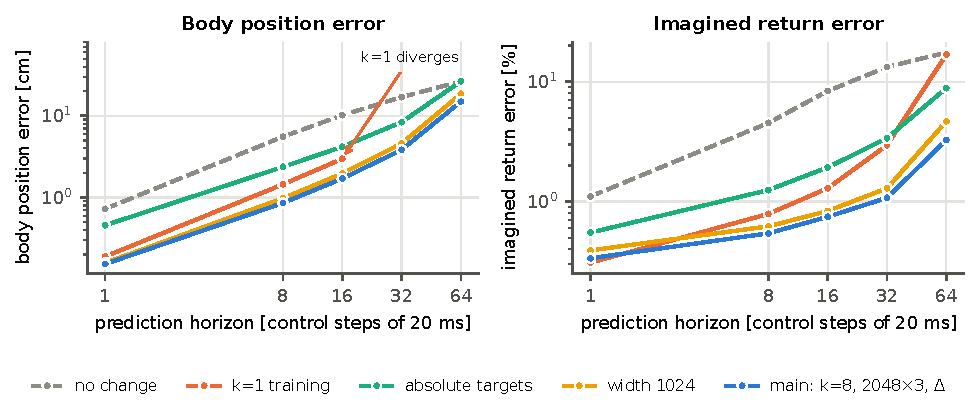
\includegraphics[width=\textwidth]{horizon.pdf}
\caption{Open-loop error on held-out clips vs prediction horizon (log scales). Left: mean world-position
error of the 14 tracked bodies. Right: relative error of the imagined tracking return. ``No change'' is
the floor; the $k{=}1$ model leaves the plot at 32 steps.}
\label{fig:horizon}
\end{figure}

\begin{table}[H]
\centering\small
\caption{Main model vs the no-change floor, held-out clips, 4096 windows per horizon. Errors at step $h$;
return error over the window.}
\label{tab:prediction}
\setlength{\tabcolsep}{4.5pt}
\begin{tabular}{lrrrrrrrrr}\toprule
predictor & $h$ & body & body p95 & arms (local) & legs (local) & root $z$ & tilt & root $xy$ & return err \\
 & steps & cm & cm & cm & cm & cm & deg & cm & \% \\\midrule
no change & 1 & 0.73 & 2.10 & 0.74 & 0.49 & 0.18 & 0.46 & 0.50 & 1.10 \\
 & 8 & 5.55 & 16.16 & 5.52 & 3.32 & 1.21 & 3.08 & 3.89 & 4.53 \\
 & 16 & 10.20 & 31.03 & 9.53 & 5.12 & 1.75 & 4.65 & 7.49 & 8.36 \\
 & 32 & 16.94 & 52.46 & 14.02 & 6.53 & 2.17 & 6.33 & 12.71 & 13.26 \\
 & 64 & 26.43 & 88.42 & 17.45 & 6.88 & 2.28 & 7.09 & 20.92 & 17.49 \\
\midrule
main ($k{=}8$, $2048{\times}3$, $\Delta$) & 1 & 0.15 & 0.32 & 0.16 & 0.12 & 0.06 & 0.08 & 0.03 & 0.34 \\
 & 8 & 0.86 & 1.82 & 1.20 & 0.56 & 0.16 & 0.49 & 0.25 & 0.54 \\
 & 16 & 1.70 & 3.57 & 2.34 & 0.93 & 0.25 & 0.85 & 0.73 & 0.75 \\
 & 32 & 3.83 & 8.19 & 4.37 & 2.11 & 0.35 & 2.06 & 2.64 & 1.08 \\
 & 64 & 14.93 & 33.05 & 10.93 & 9.03 & 1.37 & 9.45 & 14.74 & 3.26 \\
\bottomrule\end{tabular}

\end{table}

\begin{itemize}
  \item \textbf{Error grows smoothly and stays small up to 32 steps:} 0.15, 0.86, 1.7 and 3.8\,cm at 1,
  8, 16 and 32 steps. That is 4.4--6.5$\times$ below the no-change floor. At 32 steps, 95\% of windows
  are within 8.2\,cm.
  \item \textbf{The root is accurate:} 0.35\,cm in height, 2.1\textdegree{} in tilt and 2.6\,cm of
  planar drift after 32 steps.
  \item \textbf{The reward is even more accurate:} the imagined return is within 1.1\% at 32 steps. The
  exponential kernels barely react to errors of a few centimetres. What the policy needs is the
  reward's \emph{gradient}, which Q2 tests.
  \item \textbf{Beyond 32 steps the error accelerates:} 14.9\,cm at 64 steps (95th percentile 33\,cm),
  only $1.8\times$ better than no change. Every rollout stayed finite, but 64 steps is past the model's
  useful range. This agrees with the paper's $H = 32$ plus a critic for the rest.
\end{itemize}

\textbf{Where the error is (\fig{fig:groups}).}
\begin{itemize}
  \item \textbf{By group:} relative to the root, the arms carry the largest error (4.4\,cm at 32
  steps), the legs half of it (2.1\,cm), and the torso, close to the root, very little (0.24\,cm). In
  joint space, arm errors are 0.038\,rad and leg errors 0.016\,rad.
  \item \textbf{Likely reasons (untested):}
  \begin{itemize}
    \item The arms move the most in BONES-SEED motions.
    \item At 1\,Hz they are compliant: where they go depends on how the torso swings them, not only
    on their setpoint.
  \end{itemize}
  \item \textbf{Same pattern in PPO-Sim:} the arms were also the largest tracking error there
  (10.8\,cm).
\end{itemize}

\begin{figure}[H]
\centering
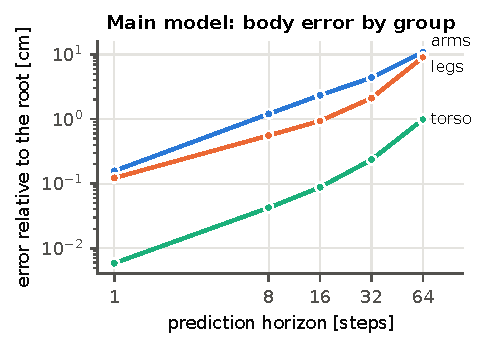
\includegraphics[width=0.48\textwidth]{groups.pdf}
\caption{Main model: body-position error relative to the root, by group, vs horizon.}
\label{fig:groups}
\end{figure}

\subsection{Q4: which design choices matter (ablations)}

Each ablation changes one thing from the main model; data, split, steps and seed are the same.
\tab{tab:ablation} and \fig{fig:horizon} compare the results on held-out clips, and \fig{fig:training}
shows the held-out losses during training.

\begin{table}[H]
\centering\small
\caption{Ablations on held-out clips: mean body error and imagined-return error. ``Diverged'': the
mean error exceeds 10\,m because a fraction of the rollouts blow up.}
\label{tab:ablation}
\begin{tabular}{lrrrrr}\toprule
 & \multicolumn{2}{c}{8 steps} & \multicolumn{2}{c}{32 steps} & 64 steps \\
\cmidrule(lr){2-3}\cmidrule(lr){4-5}\cmidrule(lr){6-6}
model & body [cm] & return [\%] & body [cm] & return [\%] & body [cm] \\\midrule
main ($k{=}8$, $2048{\times}3$, $\Delta$) & 0.86 & 0.54 & 3.83 & 1.08 & 14.9 \\
width 1024 & 0.98 & 0.62 & 4.58 & 1.29 & 18.6 \\
absolute targets & 2.37 & 1.25 & 8.36 & 3.38 & 26.4 \\
$k{=}1$ training & 1.45 & 0.79 & diverged & 2.95 & diverged \\
no change & 5.55 & 4.53 & 16.94 & 13.26 & 26.4 \\
\bottomrule\end{tabular}

\end{table}

\begin{itemize}
  \item \textbf{Single-step training ($k{=}1$) diverges.}
  \begin{itemize}
    \item After one step it is almost as good as the main model (0.19 vs 0.15\,cm). Its error then
    compounds: 1.45\,cm at 8 steps, and it diverges at 32 steps.
    \item In training, its 32-step held-out loss explodes from about 30k steps on (\fig{fig:training},
    right), while its 8-step loss keeps falling.
    \item Why: trained only on true inputs, the model never learns what to do once its own small errors
    take it off the data, so nothing holds it there.
    \item Its return error (3\%) hides the divergence, because the reward saturates at zero for
    far-off states.
  \end{itemize}
  The paper's multi-step loss is essential.
  \item \textbf{Absolute targets are $2\times$ worse.} Predicting $s_{t+1}$ directly instead of
  $s_{t+1} - s_t$ gives 0.46\,cm after one step (3$\times$ worse) and 8.4\,cm at 32 steps
  (2.2$\times$). The network must reproduce the whole state to recover a small change, and the change
  drowns in the regression error.
  \item \textbf{Width 1024 is 14--19\% worse.}
  \begin{itemize}
    \item With 2.4M instead of 8.9M parameters: 0.98\,cm at 8 steps and 4.6\,cm at 32.
    \item It trains $2.7\times$ faster (16 vs 43\,min).
    \item The main model is still improving at 50k steps (\fig{fig:training}), so more steps or data
    may still help.
  \end{itemize}
  \item \textbf{An unseen policy costs about 15\% (\tab{tab:shift}).} We trained a model without the
  iteration-4000 data and tested it on that policy's held-out clips. Error rises from 0.82 to 0.93\,cm at
  8 steps and from 3.6 to 4.2\,cm at 32. The model carries over between neighbouring policies. This is
  the situation in M3, where the policy drifts away from the data; M4's online refits close the gap.
\end{itemize}

\begin{table}[H]
\centering\small
\caption{Policy shift: held-out clips of the iteration-4000 data, for the main model (trained on it)
and a model trained only on the iteration-1000 and 8800 data.}
\label{tab:shift}
\begin{tabular}{lrrr}\toprule
model (data of the 4000-iteration policy) & body, 8 steps [cm] & body, 32 steps [cm] & return err, 32 [\%] \\\midrule
main ($k{=}8$, $2048{\times}3$, $\Delta$) & 0.82 & 3.60 & 1.02 \\
unseen policy & 0.93 & 4.18 & 1.30 \\
\bottomrule\end{tabular}

\end{table}

\begin{figure}[H]
\centering
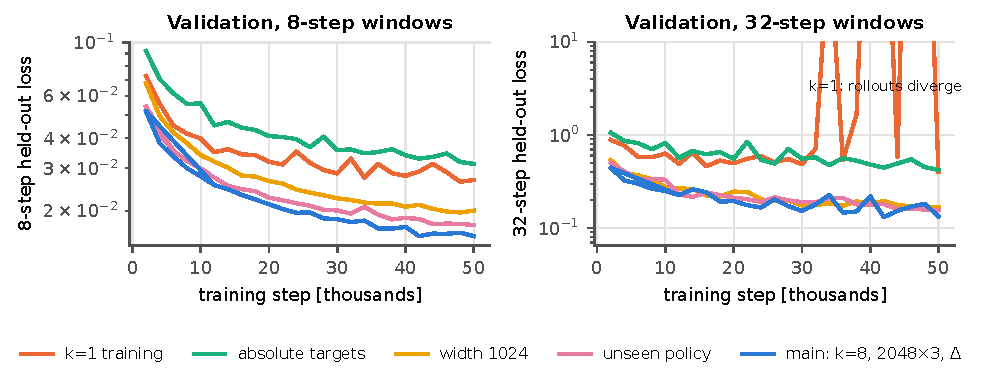
\includegraphics[width=\textwidth]{training.pdf}
\caption{Held-out losses during training (Eq.~1 without the failure term). Left: 8-step windows, the
training length. Right: 32-step windows, the policy's horizon. The $k{=}1$ model improves at 8 steps
while its 32-step rollouts diverge.}
\label{fig:training}
\end{figure}

\textbf{Not ablated.}
\begin{itemize}
  \item \textbf{The ``10 batches of 2048 windows'' reading (D10).} It sets how many model updates the
  online loop makes per environment step. Offline it has no meaning, so it moves to M4.
  \item \textbf{The normalizer ablation.} Dropped: frozen per-dimension statistics trained every
  variant smoothly, and nothing pointed at them.
\end{itemize}

\subsection{Q2: are the gradients useful?}

\begin{figure}[H]
\centering
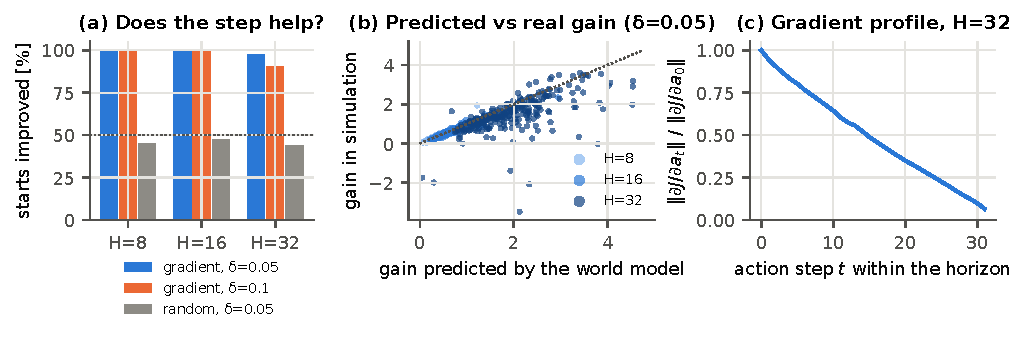
\includegraphics[width=\textwidth]{gradients.pdf}
\caption{Gradient check, main model, 256 held-out starts. (a) Share of starts whose simulated return
improved after a step along the model's gradient vs a random direction of the same size. (b) Gain
predicted by the model vs gain measured in simulation, per start ($\delta = 0.05$); the dotted line is
$y = x$. (c) Gradient norm per action step along a 32-step horizon, relative to the first step.}
\label{fig:gradients}
\end{figure}

\begin{table}[H]
\centering\small
\caption{Gradient check: share of improved starts, mean return gain predicted by the model and
measured in simulation, and their correlation across starts. Random: mean of two directions,
$\delta = 0.05$.}
\label{tab:gradients}
\begin{tabular}{rrrrrrrrr}\toprule
 & \multicolumn{3}{c}{starts improved [\%]} & \multicolumn{3}{c}{$\delta=0.05$} & \multicolumn{2}{c}{$\delta=0.1$} \\
\cmidrule(lr){2-4}\cmidrule(lr){5-7}\cmidrule(lr){8-9}
$H$ & grad $0.05$ & grad $0.1$ & random & predicted & real & corr & predicted & real \\\midrule
8 & 100 & 100 & 45 & 0.24 & 0.23 & 0.95 & 0.43 & 0.41 \\
16 & 100 & 100 & 47 & 0.68 & 0.63 & 0.96 & 1.18 & 1.07 \\
32 & 97 & 90 & 44 & 1.98 & 1.50 & 0.62 & 2.70 & 1.72 \\
\bottomrule\end{tabular}

\end{table}

\begin{itemize}
  \item \textbf{Direction: the gradient is right almost every time.}
  \begin{itemize}
    \item At $H = 8$ and 16, every gradient step improved the simulated return.
    \item At $H = 32$: 97\% of starts improved for $\delta = 0.05$, and 90\% for $\delta = 0.1$.
    \item Random directions improved 44--47\%. The logged actions come from a trained policy, so a
    random change hurts slightly more often than it helps.
  \end{itemize}
  \item \textbf{Size: accurate up to 16 steps, optimistic at 32.}
  \begin{itemize}
    \item Up to 16 steps the predicted gain is within 10\% of the real one, and the two correlate at
    0.95--0.97 across starts.
    \item At 32 steps the model predicts 1.98 where the simulator gives 1.50 ($\delta = 0.05$, +32\%),
    and 2.70 vs 1.72 ($\delta = 0.1$, +57\%). The correlation drops to 0.62--0.72.
    \item The larger the step, the larger the optimism. This is the classic failure mode of model-based
    RL: an optimizer finds the actions where the model errs in its own favour. The policy update in M3
    is exactly such an optimizer.
  \end{itemize}
  \item \textbf{Gradient flow: no explosion, no vanishing} (\fig{fig:gradients}c).
  \begin{itemize}
    \item The norm of $\partial J/\partial a_t$ decays smoothly and almost linearly along the horizon,
    from 0.54 at $t = 0$ to 0.035 at $t = 31$.
    \item An action at step $t$ can only affect the $H - t$ rewards after it, so a linear decay is what
    well-behaved dynamics give.
    \item Exploding gradients would grow faster than linearly toward $t = 0$; vanishing gradients would
    collapse within a few steps. Neither happens.
  \end{itemize}
\end{itemize}

The gains are small next to the return (1.5 of about 98 at $H=32$) because the steps are deliberately
small, i.e.\ first order. The test is about direction, and the direction is right.

\subsection{Q3: predicting failures}

\begin{figure}[H]
\centering
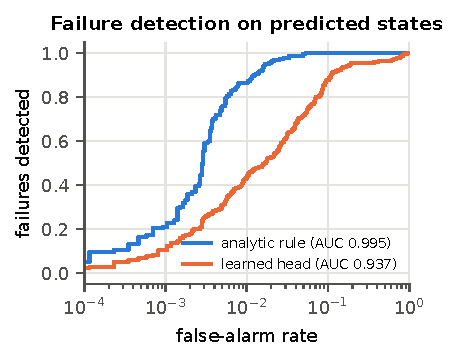
\includegraphics[width=0.48\textwidth]{termination.pdf}
\caption{Failure detection on the main model's predicted states, held-out clips (log false-alarm axis).
The analytic rule is the env's own failure definition applied to the predicted state.}
\label{fig:termination}
\end{figure}

\begin{itemize}
  \item \textbf{The learned head misses the gate:} AUC 0.937, against a gate of 0.95. The other models
  score 0.91--0.95, except $k{=}1$ at 0.71.
  \item \textbf{The env's rule on the same predicted states scores 0.995} (0.97--0.996 across models).
  \item \textbf{Under policy shift} the head drops to 0.872 for the model that never saw the policy,
  while the rule stays at 0.997.
  \item \textbf{The fault is the head, not the states.} A larger check with 20$\times$ negatives gives
  the head 0.961 on predicted states and 0.954 on \emph{true} states. Given perfect states, it is still
  worse than the rule.
  \item \textbf{The rule as a hard threshold} ($m > 1$) catches 81\% of failures at the exact step, at
  a false-alarm rate of 0.02\%.
\end{itemize}

\textbf{Why the head struggles.} Failures are 0.05\% of transitions. The label is a sharp threshold
on two quantities. Cross-entropy is minimized by answering a confident ``no failure'' almost
everywhere: the held-out failure loss sits near $10^{-4}$ while the ranking stays mediocre. The rule,
in contrast, \emph{is} the definition of the label, and the predicted states are accurate enough to
apply it.

\subsection{Gates}

\begin{table}[H]
\centering\small
\caption{M2 gates (main model, held-out clips).}
\label{tab:gates}
\begin{tabular}{llll}\toprule
question & gate & measured & \\\midrule
Q1 & 8-step body error $< 2$\,cm mean, $< 5$\,cm p95 & 0.86 / 1.82\,cm & pass \\
Q1 & 32-step rollouts bounded, body error $< 10$\,cm & 3.83\,cm, all finite & pass \\
Q1 & imagined return error $< 10\%$ at 32 steps & 1.1\% & pass \\
Q2 & gradient steps beat random directions & 90--100\% vs 44--47\% & pass \\
Q3 & failure AUC $> 0.95$ & head 0.937 / rule 0.995 & head fails, rule passes \\
Q4 & $k{=}8$ beats $k{=}1$ & 3.8\,cm vs diverged at 32 steps & pass \\\bottomrule
\end{tabular}
\end{table}

\section{Decisions for M3}

\begin{enumerate}
  \item \textbf{World model:} the main configuration: $k = 8$, $2048{\times}3$ ELU, delta targets,
  frozen normalization, trained on all three data sets
  (\texttt{logs/supermimic\_m2/wm/main/wm\_best.pt}).
  \item \textbf{Failure probability in imagination: a smooth analytic rule}, in place of the learned
  head:
  $\hat d = \sigma\big((m(\hat s, g) - 1)/\tau\big)$ with $\tau \approx 0.05$.
  \begin{itemize}
    \item It is differentiable, so the survival weight still pushes the policy away from falls.
    \item It has no parameters to fit, and it does not degrade under policy shift.
    \item It deviates from the paper, which learns $d_\omega$. The learned head stays in the model and
    in the logs, so M3 can compare the two.
  \end{itemize}
  \item \textbf{Guard against model optimism} at $H = 32$:
  \begin{itemize}
    \item Log the imagined vs simulated return of the same policy from the first iteration.
    \item Keep the paper's small policy steps: learning rate $2\cdot10^{-4}$, gradient clipping at a
    global norm of 1.0 and then 0.1 per element.
    \item If the gap grows, ablate $H = 16$, where the gradients were accurate.
  \end{itemize}
  \item \textbf{Watch the arms.} They carry the largest model error, and they were already the weakest
  part of the PPO baseline.
\end{enumerate}

\section{Next steps}

\textbf{M3: a policy on the frozen world model.} Build:
\begin{itemize}
  \item \textbf{Imagination:} roll out from replay start states, with the previous 9 logged steps to
  fill the 10-frame observation history.
  \begin{itemize}
    \item Observations are computed from the predicted state (actuated joints only, D28), with the
    sensor noise added back as in the paper.
    \item Goals are the next 10 reference frames from the motion library.
    \item Clip ends are handled as in D8.
  \end{itemize}
  \item \textbf{Objective:} Eq.~2 with the survival weight, plus the critic trained on $\lambda$-returns
  (Eq.~3: $\lambda = 0.95$, $\gamma = 0.99$, 5 epochs of 4 minibatches).
  \item \textbf{Optimizers:} the paper's, Adam with $\beta = (0.9, 0.95)$ for the policy.
  \item \textbf{Evaluation:} the policy in the simulator every few hundred iterations, with
  \texttt{eval.py} on \texttt{dev}, next to its imagined return.
\end{itemize}

\textbf{Runs, in this order:}
\begin{enumerate}
  \item \textbf{Warm start from the PPO-Sim actor} (same encoder--decoder network, D17), $H = 32$ with
  the critic. This is the policy-level version of the gradient check: do world-model updates improve a
  good policy in the simulator? It stays close to the data the model was trained on.
  \item \textbf{The same without the critic}, which is the roadmap's comparison.
  \item \textbf{From scratch on the frozen model.} This is a stress test: a fresh policy leaves the data
  distribution quickly, and the paper only ever trains online.
\end{enumerate}

\textbf{M3 gate:} the simulated return follows the imagined one, and the critic run beats the
no-critic run.

\textbf{M4} then closes the loop as in the paper: about 2.5 simulator steps per iteration, model
refits, one policy step and one critic fit. It is compared with PPO-Sim on wall-clock time to a target
return.

\appendix
\section{Settings and compute}

\begin{table}[H]
\centering\small
\begin{tabular}{ll}\toprule
\multicolumn{2}{l}{\textbf{World model}} \\
state / action / context dims & 77 / 28 / 32 \\
dynamics MLP & $3\times2048$, ELU; 80 outputs (state change + heading-frame pose change) \\
termination MLP & $2\times256$, ELU; inputs: state + reference root height and $g_z$ \\
normalization & per dimension, from 200k training transitions, frozen \\
pose loss scales & 0.1\,m, 0.1\,rad \\
\multicolumn{2}{l}{\textbf{Training}} \\
windows & $k = 8$, never across an episode end \\
optimizer & Adam, lr $2\cdot10^{-4}$, batch 2048 windows, gradient-norm clip 1.0, TF32 \\
steps & 50k; keep the best held-out 8-step loss (main: step 42k) \\
\multicolumn{2}{l}{\textbf{Data}} \\
policies & PPO-Sim (1\,Hz arms/waist) at iterations 1000, 4000, 8800 \\
per policy & 4096 envs $\times$ 500 steps, action noise $\mathcal N(0, 0.1^2)$, paper DR per episode \\
library / held-out & \texttt{dev} (1296 clips, 2.56\,h) / 118 clips by name hash \\
\multicolumn{2}{l}{\textbf{GPU time} (RTX 5060 Ti 16\,GB, shared)} \\
collection & 2\,min \\
training & main 43, $k{=}1$ 6, width 1024 16, absolute 43, unseen policy 43\,min \\
evaluation & 1\,min open loop (all models), 33\,s gradient check \\\bottomrule
\end{tabular}
\end{table}

\section{Reproduction}

From the worktree root; GPU jobs go through the queue (\texttt{gpu-run}). Write the data paths out
in full: the queue's shell does not split a variable into several arguments.
\begin{small}
\begin{verbatim}
D="logs/supermimic_m2/data"; P="logs/rsl_rl/supermimic_ppo_sim_1hz/2026-10-22_21-11-56"
# 1. data (2 min)
python -m pal_mjlab.scripts.supermimic.collect_rollouts \
  --task Mjlab-SuperMimic-PPO-Flat-Pal-Kangaroo-Grippers-ArmWaist1Hz \
  --checkpoints $P/model_1000.pt $P/model_4000.pt $P/model_8800.pt --out-dir $D
# 2. models (main; ablations add --k 1 | --hidden 1024 1024 1024 | --no-predict-delta
#    | --train-sources model_1000 model_8800)
python -m pal_mjlab.scripts.supermimic.train_world_model \
  --data $D/model_1000 $D/model_4000 $D/model_8800 --out-dir logs/supermimic_m2/wm/main
# 3. open-loop evaluation and failure AUC (add --sources model_4000 for the policy shift)
python -m pal_mjlab.scripts.supermimic.eval_world_model \
  --models main=logs/supermimic_m2/wm/main/wm_best.pt k1=... \
  --data $D/model_1000 $D/model_4000 $D/model_8800 --out-json logs/supermimic_m2/eval/all.json
# 4. gradient check
python -m pal_mjlab.scripts.supermimic.grad_check --model logs/supermimic_m2/wm/main/wm_best.pt \
  --data $D/model_1000 $D/model_4000 $D/model_8800 --out-json logs/supermimic_m2/eval/grad_main.json
# 5. figures, tables, this report
python docs/supermimic/m2/make_figures.py && (cd docs/supermimic/m2 && latexmk -pdf report.tex)
\end{verbatim}
\end{small}

\textbf{Code.}
{\raggedright
\begin{itemize}
  \item Model and data: \texttt{state.py}, \texttt{rl/world\_model.py} and \texttt{rl/replay.py} in
  \texttt{src/pal\_mjlab/tasks/supermimic/}.
  \item Scripts: \texttt{collect\_rollouts.py}, \texttt{train\_world\_model.py},
  \texttt{eval\_world\_model.py} and \texttt{grad\_check.py} in
  \texttt{src/pal\_mjlab/scripts/supermimic/}.
  \item Tests: \texttt{tests/supermimic/test\_world\_model.py}. They cover the state round trip, windows
  inside episodes, overfitting a batch, gradients against finite differences, and reward parity on
  collected data.
\end{itemize}
}

\end{document}
